\section{First prototype} \label{ch:first_prototype}

To create a first prototype capable of detecting hand-drawn mechanism, various capabilities have to be considered.
The application has to be able to detect \name{nodes}, \name{constraints}, which are connecting \name{nodes} and to transform this information into a usable format.

\subsection{The Fully Connected Convolutional Neural Network}.

The topic of a previous work was the recognition of hand-drawn mechanical symbols \cite{Lawrence2020}.
Building on this, the trained model is improved to provide not only the class, but the location of the classification in an image of arbitrary size.

The respective model can be loaded using \name{Keras'}, % TODO citation should be in the introduction.
\code{model.load\_model} and by issuing the \code{summary} method we get listing~\ref{lst:srp_model}.

\begin{lstlisting}[caption={Summary of Symbol Classifier}, label={lst:srp_model}]
_________________________________________________________________
Layer (type)                 Output Shape              Param #
=================================================================
conv2d (Conv2D)              (None, 32, 32, 16)        272
_________________________________________________________________
max_pooling2d (MaxPooling2D) (None, 16, 16, 16)        0
_________________________________________________________________
conv2d_1 (Conv2D)            (None, 16, 16, 32)        8224
_________________________________________________________________
max_pooling2d_1 (MaxPooling2 (None, 8, 8, 32)          0
_________________________________________________________________
flatten (Flatten)            (None, 2048)              0
_________________________________________________________________
dense (Dense)                (None, 3)                 6147
=================================================================
Total params: 14,643
Trainable params: 14,643
Non-trainable params: 0
_________________________________________________________________
\end{lstlisting}

One way to localize images in a bigger image is to scan each sector of an image and predicting the generated crops.
Using a 360x360 sized image, a stride of one in each direction, the number of images which are used in the prediction process are 108.241 images\footnote{$h + 1 - 32 * w + 1 - 32$, where $h$ and $w$ are the height and width of the input image and the size of the kernel used to predict is 32}.
A Jupyter notebook to test the performance on this can be found at \url{https://aka.klawr.de/sep#1}. % TODO Set this URL.

To test this amount of images is often not necessary and can be reduced by increasing the stride of the respective scanning process.
This would reduce the accuracy of the localization, but would increase the speed.

Another approach is to use the properties of convolutional layer to restructure the model and thereby making the whole procedure much more efficient.

By transforming a model into a Fully Connected Convolutional Neural Network (FCN) all dense layers are replaced by convolutional layers, and the input layer is also a two dimensional layer but allows for an input image of arbitrary size.
Because the input of the original model is only defined by the kernel size, it is agnostic to the size of a previous layer.
Listing \ref{lst:to_fcn} transforms the \code{old\_model} by appending an \code{tf.keras.Input} layer without any specified size and replacing the output layer by a \code{tf.keras.Conv2D} layer\footnote{And thus removing the \code{tf.keras.flatten} layer.}

\begin{lstlisting}[caption={Transformation into a FCN}, label=lst:to_fcn]
inputs = tf.keras.Input(shape=(None, None, 1))

hidden = old_model.layers[0](inputs)

for layer in old_model.layers[1:4]:
    hidden = layer(hidden)

# Get the input dimensions of the flattened layer:
f_dim = old_model.layers[4].input_shape
# And use it to convert the next dense layer:
dense = old_model.layers[5]
out_dim = dense.get_weights()[1].shape[0]
W, b = dense.get_weights()
new_W = W.reshape((f_dim[1], f_dim[2], f_dim[3], out_dim))
outputs = tf.keras.layers.Conv2D(out_dim,
                           (f_dim[1], f_dim[2]),
                           name = dense.name,
                           strides = (1, 1),
                           activation = dense.activation,
                           padding = 'valid',
                           weights = [new_W, b])(hidden)

model = tf.keras.Model(inputs = inputs, outputs = outputs)

model.summary()
\end{lstlisting}

An example for the usage of this code can be found at \url{https://aka.klawr.de/sep#2} % TODO
, where the intricate differences between both approaches are discussed.

The FCN approach is roughly ten times faster than taking crops and predicting them individually. 
This \code{model.summary} results in the following output:

\begin{lstlisting}
Model: "model"
_________________________________________________________________
Layer (type)                 Output Shape              Param #   
=================================================================
input_1 (InputLayer)         [(None, None, None, 1)]   0         
_________________________________________________________________
conv2d (Conv2D)              multiple                  272       
_________________________________________________________________
max_pooling2d (MaxPooling2D) multiple                  0         
_________________________________________________________________
conv2d_1 (Conv2D)            multiple                  8224      
_________________________________________________________________
max_pooling2d_1 (MaxPooling2 multiple                  0         
_________________________________________________________________
dense (Conv2D)               (None, None, None, 3)     6147      
=================================================================
Total params: 14,643
Trainable params: 14,643
Non-trainable params: 0
_________________________________________________________________
\end{lstlisting}

Granted this model is satisfactory for the moment, the problem of detecting constraints can be addressed.

\subsection{Constraint detection}

There was already a model providing the capability of detecting symbols, to prior work.
To create a model for detecting constraints the same procedure has to be followed, which means that training data has to be generated first.

\subsubsection{Data generation}

It is planned to support two different constraints, which indicate whether two nodes are either able to rotate around one another or to be able to move in a translational fashion.
Besides different types of constraints one of three different ranges can be selected for the length of the respective constraint.

Data generation for constraints is similar to data generation in \cite{Lawrence2020}.
The drawing canvas has a width of fifty and the range can vary between 150-249, 250-349 or 350-449; depending on the selected range.

\begin{figure}
    \centering
    \begin{subfigure}[b]{0.45\textwidth}
        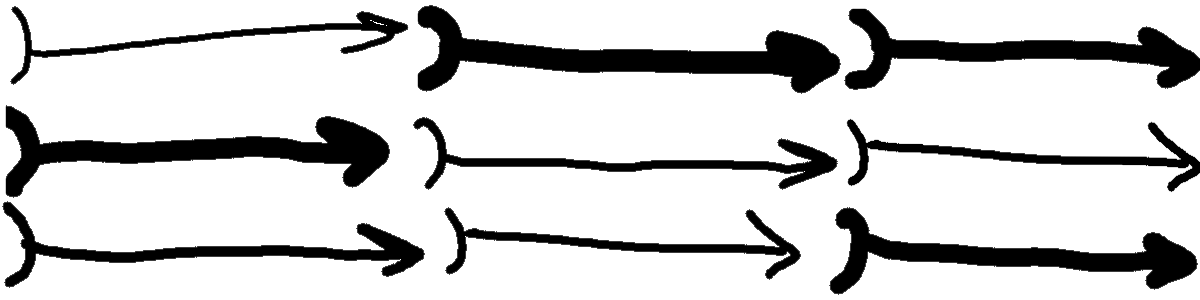
\includegraphics[width=\textwidth]{images/rs.png}
        \caption{Rotational Constraints}
        \label{fig:rotational_constraints}
    \end{subfigure}
    \begin{subfigure}[b]{0.45\textwidth}
        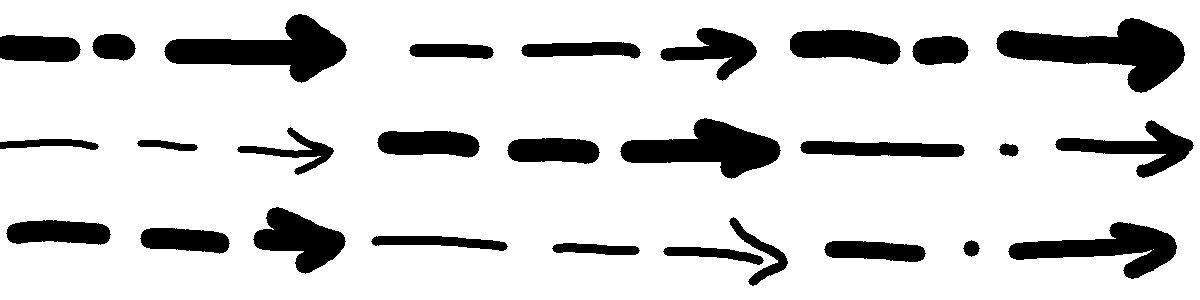
\includegraphics[width=\textwidth]{images/ts.png}
        \caption{Translational Constraints}
        \label{fig:translational_constraints}
    \end{subfigure}
    \caption{Some examples of the data created with the described method. Only these two classes were created for the first tests. The images are created horizontally, so their initial angle can be assumed to be zero to keep record when labeling the data dynamically. }
    \label{fig:generated_data_samples}
\end{figure}

Since constraints can occur at all possible angles, the data must be generated in such a way that it resembles the reality the most.

The first step is to randomly place nodes in images, which can then be connected using the generated constraints.
For this two different interim datasets have been created resembling these two steps.
% TODO get code which does this and put it into /reports/sep/code
